\section{Разработка программного средства}

В данном разделе будет описан процесс проектирования и программирования основных
модулей программного средства

\subsection{Общее описание архитектуры}
С целью обеспечения гибкости архитектуры и модульности, принято решение разбить
функционал программного средства на следующие \mbox{модули}:
\begin{itemize}
  \item набор модулей для работы с сетью на уровне запросов;
  \item модуль для работы с API \vk{}.
  \item модуль для работы с LongPoll сервером;
  \item модуль для хранения кэша загруженных данных и обеспечения связи с
  графическим интерфейсом;
  \item база данных для сохранения кэша на диск;
  \item модуль для взаимодействия с базой данных;
  \item набор классов для представления различных типов данных, используемых API
  социальной сети;
  \item набор модулей для реализации графического интерфейса.
\end{itemize}

Учитывая специфику асинхронной работы с сетью, важным моментом является логика
обновления данных в представлении. Обновление данных может происходить в разном
порядке по мере загрузки информации из сети. Кроме события получения новых
сообщений в фоновом режиме возможно обновление фотографии пользователя,
онлайн-статуса собеседника, статуса прочитанности сообщений и многой другой
информации. Всё это должно не только своевременно отражаться в графическом
интерфейсе, но и выборочно сохраняться в локальный кэш, который необходим для
сокращения времени синхронизации с данными учётной записи.

Для решения обозначенной проблемы предназначен модуль хранения кэша загруженных
данных, являющийся связующим звеном между модулями для работы с сетью,
графическим интерфейсом и базой данных для сохранения кэша в постоянной памяти.

Взаимодействие хранилища и графического интерфейса осуществляется с применением
паттерна <<Наблюдатель>>. Хранилище обрабатывает постоянно загружаемые из сети
данные и в случае необходимости уведомляет графический интерфейс об обновлении,
что в свою очередь вызывает перерисовку нужных элементов.

С целью ослабления зависимостей между графическим интерфейсом и подсистемой
работы с сетью создан модуль для работы с API \vk{}, инакпсулирующий всю
необходимую работу с сетью через соответствующие модули.

Такая декомпозиция помогает упростить процесс разработки и обеспечивает
возможность независимой работы над различными функциональными компонентами
программного средства.

\subsection{Работа с сетью}
Qt предлагает набор классов для удобной асинхронной работы с сетью с
использованием сигнально-слотовой системы. Для загрузки определенной
веб-страницы необходимо организовать взаимодействие объектов трёх классов:
QNetworkAccessManager, QNetworkRequest и QNetworkReply.

Класс QNetworkAccessManager позволяет выполнять сетевые запросы, представляемые
объектами класса QNetworkRequest и получать ответы на них в виде загруженных
данных. Объект данного класса хранит сетевые настройки для запросов, которые
будут отправляться с его помощью. Для обработки загруженных данных в классе
имеется сигнал replyFinished, передающий объект класса QNetworkReply, содержащий
все загруженные данные. Пример кода, иллюстрирующий данное описание, представлен
в листинге \ref{lst:load_page}.

\begin{lstlisting}[style = cstyle, 
				   caption = {Загрузка страницы с использованием Qt},
				   label = lst:load_page] 
QNetworkAccessManager *manager = new QNetworkAccessManager(this);
connect(manager, SIGNAL(finished(QNetworkReply*)),
 	  this, SLOT(replyFinished(QNetworkReply*)));
manager->get(QNetworkRequest(QUrl("http://vk.com")));
\end{lstlisting}

Работа с сетью в программе осуществляется следующим набором классов:
\begin{itemize}
  \item VNetworkManager --- основной класс для работы с сетью, объединяющий при
  помощи механизма композиции более узкоспециализированные классы;
  \item VNetworkLongPoll --- класс для работы с LongPoll сервером;
  \item VNetworkSimple --- класс, предназначенный для выполнения обычных
  GET запросов;
  \item VNetworkReply --- вспомогательный класс, используемый в
  классе VNetworkSimple для обработки загруженных данных.  
\end{itemize}

Разделение функционала данных классов и классов, выполняющих обработку
загруженных данных, достигается при помощи системы сигналов и слотов Qt.
Схема соединения сигналов и слотов, обеспечивающих обновление интерфейса,
приведена на рисунке \ref{fig:network_signals_slots}.

\begin{figure}
\centering
	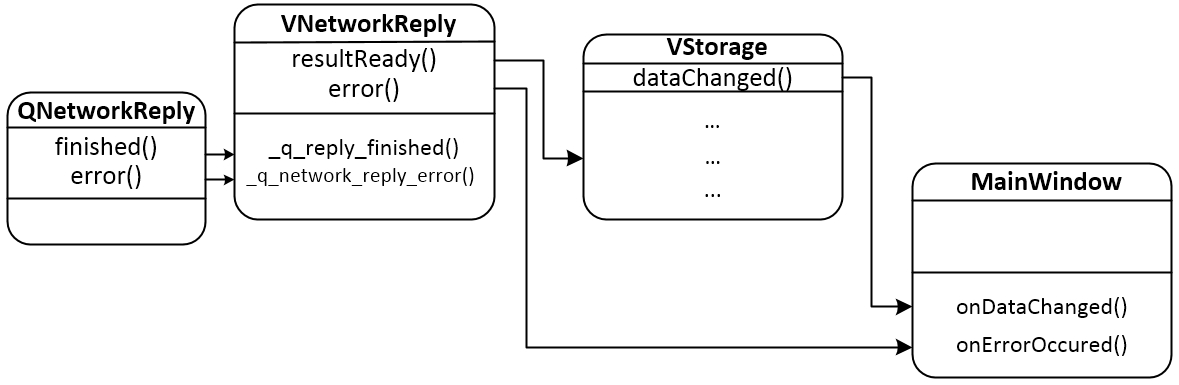
\includegraphics[scale = 0.52]{network_signals_slots.jpg}
	\caption{Схема соединения сигналов и слотов, \\ обеспечивающих обновление
	интерфейса}
	\label{fig:network_signals_slots}
\end{figure}

Из приведённой схемы видно, что библиотечный класc QNetworkReply связан с
VNetworkReply. Такая агрегация позволяет выполнить предварительную
низкоуровневую обработку ответа перед тем, как передавать его в класс,
обеспечивающий кэширование. На данном этапе происходит создание JSON-объекта,
используемого другими модулями программы, и отслеживание некоторых типов ошибок.
Многоточия на схеме обозначают набор слотов, с одним или несколькими из которых
будет соединён сигнал resultReady класса VNetworkReply. Выбор данного слота
осуществляется в зависимости от типа загружаемых данных. В то же время выработка
сигнала dataChanged от типа обновлённой информации зависит лишь вспомогательными
для интерфейса данными, которые передаются в качестве параметров функции.

Доступа к методам классов VNetworkManager и доступных из него VNetworkSimple и
VNetworkLongPoll организован с использованием паттерна <<Одиночка>>.
Данный паттерн обеспечивает наличие единственного экземпляра класса с глобальной
точкой доступа в однопоточном приложении. Класс VNetworkManager гарантирует это
благодаря классическому для C++ приёму, называемому синглтон Майерса: в
публичном методе getInstance() объявляется статическая переменная, имеющая тип
данного класса, а конструктор класса переносится в секцию private. Дополнительно
к этому запрещается использование конструктора копий и оператора присваивания,
для этого применяется ключевое слово delete, введенное в стандарте С++11.
Похожим образом в классе VNetworkManager организован доступ к классу для
выполнения простых GET запросов и классу для работы с LongPoll сервером. В
качестве примера в листинге \ref{lst:vnetworksimple} приведен код для получения
экземпляра класса VNetworkSimple.

\begin{lstlisting}[style = cstyle, 
				   caption = {Получение экземпляра класса VNetworkSimple},
				   label = lst:vnetworksimple] 
VNetworkSimple *VNetworkManager::simple()
{
	static VNetworkSimple networkSimpleInstance;
	return &networkSimpleInstance;
}
\end{lstlisting}

Класс хранения static гарантирует, что переменная, объявленная таким образом,
будет создана и инициализирована только один раз перед первым использованием.
Применительно к объекту это означает, что конструктор соответствующего
класса будет вызван только один раз.

\subsection{Обработка запросов к API}

Для получения информации о состоянии учетной записи и поддержки данной
информации в актуальном состоянии требуется совершать большое число
запросов к API социальной сети, причем данные запросы могут находится в тесной
связи друг с другом.

Необходимость отправки нового запроса может возникнуть не только по команде от
пользовательского интерфейса, но и в процессе обработки другого запроса.
Также их результаты могут по-разному обрабатываться в зависимости от текущего
состояния программы и статуса завершенности зависимых запросов.

Все перечисленные факторы хорошо учитываются при организации запросов в виде
дерева.
Каждый запрос представлен узлом дерева. Дочерние узлы дерева представляют,
соответственно, зависимые запросы. Сигнал о завершении запроса не инициируется
до тех пор, пока не завершатся все его дочерние запросы, даже в том случае,
когда сам запрос уже завершился.
Реализация данной модели значительно упрощается благодаря сигнально-слотовой
системе фреймворка Qt.

По завершении запроса возможно три варианта развития событий:
отсутствие действий, уведомление представления, изменение модели. В соответствии
с данными вариантами узлы дерева, представляющие запросы, имеют три типа.
Зависимости от типа запроса, узел дерева может хранить дополнительную
информацию, необходимую для корректной реакции на его завершение. Например,
возможно уведомление представления о следующих событиях: отправка сообщения,
получение нового сообщения, удаление сообщения, загрузка аватара пользователя,
получение информации о необходимости заполнения капчи, загрузка изображения
капчи и т. д.

\subsection{Использование системы ресурсов Qt}
Система ресурсов Qt – платформо‑независимый механизм для внедрения двоичных
файлов в исполняемый файл приложения --- систему ресурсов. Это полезно, если для
разрабатываемого программного средства всегда требуется определённый набор
файлов, например, пиктограмм, файлов перевода и так далее, при этом риск потери
файлов необходимо свести к минимуму.
Ресурсы, связанные с приложением, указываются в файле коллекции ресурсов,
имеющем расширение qrc. Формат файла основан на XML, в котором перечисляются
файлы на диске и опционально присваивает им имя ресурса, используемое
приложением для доступа к ресурсу. Листинг \ref{lst:qrc_example} показывает пример файла
коллекции ресурсов:

\begin{lstlisting}[style = cssstyle, 
				   caption = {Пример файла qrc},
				   label = lst:qrc_example] 
<!DOCTYPE RCC><RCC version="1.0"> 
	<qresource>
	     <file>images/copy.png</file> <file>images/cut.png</file>
	     <file>images/delete.png</file>
	</qresource>
 </RCC>
\end{lstlisting} 

Файлы ресурсов, перечисленные в коллекции ресурсов, являются частью дерева
исходников приложения. Указываемые пути являются относительными к каталогу,
содержащему файл qrc, при этом перечисленные файлы ресурсов должны располагаться
в том же каталоге, что и файл коллекции, или в одном из подкаталогов.
Данные ресурса могут либо быть скомпилированы в двоичном виде и таким образом к
ним можно получить доступ непосредственно в коде приложения, либо двоичный
ресурс может быть создан и станет возможно позже ссылаться на него в коде
приложения зарегистрированный с помощью системы ресурсов.

В листинге \ref{lst:stylesheet_load} демонстрируется метод, используемый для
загрузки стиля QSS из ресурса.
\begin{lstlisting}[style = cstyle, 
				   caption = {Загрузка стиля для виджета из файла},
				   label = lst:stylesheet_load] 
void VHelper::loadStyleSheetFromFile(QString fileName, QWidget *target)
{
    QFile styleSheetFile(fileName);
    if (styleSheetFile.open(QIODevice::ReadOnly) )
    {
        QString qss = QLatin1String(styleSheetFile.readAll() );
        target->setStyleSheet(qss);
        styleSheetFile.close();
    }
}
\end{lstlisting}

\subsection{Разработка графического интерфейса}

При разработке графического интерфейса важно учитывать стилистические
особенности оформления сайта и официальных клиентов \vk{}. Все они выдержаны в
одном стиле и в одной цветовой гамме, которые следует использовать и в \vkapp{}.

Для оформления графического интерфейса использовалась технология QSS, описанная
в подразделе \ref{sec:qt}. В качестве примера в листинге
\ref{lst:css_login_button} приведён стиль для оформления кнопки входа.

\begin{lstlisting}[style = cssstyle, 
				   caption = {QSS-стиль для оформления кнопки входа},
				   label = lst:css_login_button] 
QPushButton#buttonLogin {
	font-weight: 700;
	color: #fff;
	background-color: #6182aa;
	border-radius: 4px;
	padding-left: 3px;
	padding-right: 3px;
	padding-top: 8px;
	padding-bottom: 8px;
}
\end{lstlisting}

Результат применения данного стиля приведён на рисунке \ref{fig:login_button}.
Такое оформление в точности соответствует стилистике социальной сети.

\begin{figure}[h]
\centering

\includegraphics{login_button.png}
\caption{Кнопка входа, оформленная с использованием CSS}
\label{fig:login_button}
\end{figure}

Отображение сообщений и списка диалогов является более сложной задачей из-за
отсутствия готового компонента в библиотеке виджетов Qt. Для решения проблемы
необходимо создание своего виджета, отображающего всю необходимую информацию в
подходящей форме. 

За отображение сообщений в диалогах отвечает класс VMessageView,
использующий QCustomWidget и QCustomLabel. Вспомогательные классы предназначены
для переопределения некоторых виртуальных методов, необходимых для обеспечения
визуального отклика на действия пользователя. Данные методы принимают в качестве
параметров объекты служебных классов QEvent, QMouseEvent и QPaintEvent. Для
реализации необходимых эффектов потребовалось переопределить следующие
виртуальные методы родительского класса QWidget:
\begin{itemize}
  \item mousePressEvent --- метод, обрабатывающий события клика мышью по
  виджету;
  \item enterEvent и leaveEvent --- методы, в которых производится обработка
  наведения курсора мыши на виджет;
  \item paintEvent --- метод, вызывающийся при необходимости перерисовки
  виджета.
\end{itemize}

Изменение цвета сообщения по наведению мыши достигается за счёт переопределения
enterEvent и leaveEvent, а для выделения по клику используется
пользовательский обработчик mousePressEvent.

Внешний вид получившегося виджета в разных состояниях приведён на рисунке
\ref{fig:msg_style}.

\begin{figure}[h]
\centering
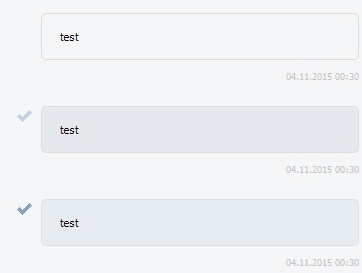
\includegraphics{msg_style.png}
\caption{Виджет для отображения сообщения в разных состояниях}
\label{fig:msg_style}
\end{figure}

Полученные виджеты удобно добавлять в любой контейнер наподобие QGridLayout для
отображения истории сообщений.

Аналогичный подход используется и для отображения списка недавних диалогов.
Каждый диалог представляется пунктом меню, содержащим имя собеседника и его
изображение профиля. Класс VDialogView реализует необходимый виджет, используя
вспомогательный класс VAvatarWidget, используемый для отображения изображения
пользователя в характерном для \vk{} стиле. Готовый виджет, отображающий
тестовые данные, приведён на рисунке \ref{fig:dialog_view}.

\begin{figure}[h]
\centering

\includegraphics{dialog_view.jpg}
\caption{Виджет для отображения информации о диалоге}
\label{fig:dialog_view}
\end{figure}

Для отображения списка диалогов, как и в случае с историей сообщений, удобно
воспользоваться компонентом QGridLayout.

Для хранения необходимых для графического интерфейса файлов изображений и QSS
стилей используется система ресурсов Qt, описанная в подразделе \ref{sec:qt}.
Такой подход позволяет сэкономить время на сборку программы и упростить
оформление графического интерфейса.

Стоит отметить, что тонкая настройка внешнего вида с помощью CSS доступна
и для созданных описанным способом пользовательских виджетов, так как они
являются объединением уже имеющихся стандартных органов управления.

Такой способ отображения сообщений и списка диалогов отличается
гибкостью и расширяемостью. При добавлении новых типов отображаемых в сообщениях
вложений можно будет сконцентрироваться на реализации нового функционала без
необходимости внесения существенных изменений в существующий код.

\subsection{Кэширование с использованием базы данных SQLite}

В подразделе \ref{sec:sqlite} описываются достоинства базы данных SQLite,
позволяющие использовать её в качестве хранилища кэша.

Qt содержит все необходимые классы для работы с различными базами данных.
Основным таким классом является QSqlDatabase, служащий для представления связи с
базой данных. В связи с тем, что низкоуровневые механизмы работы с различными
базами данных могут существенно отличаться, QSqlDatabase исользует класс
QSqlDriver. Данный класс уже зависит от используемой базы данных, однако вручную
адаптировать его придётся только в случае использования экзотических баз данных,
драйверы для которых ещё не реализованы. Стандартной библиотекой
Qt поддерживаются базы данных следующих типов:
\begin{itemize}
  \item IBM DB2;
  \item Borland InterBase Driver;
  \item MySQL;
  \item Oracle Call Interface Driver;
  \item ODBC;
  \item PostgreSQL;
  \item SQLite;
  \item Sybase Adaptive Server.
\end{itemize}

Для работы с базой данных в программе используется пользовательский класс
VStorageDatabase, инкапсулирующий всю работу с базой для загрузки или сохранения кэша.

Для подключения к существующему файлу базы данных используется статический метод
addDatabase класса QSqlDatabase, одна из версий которого принимает в качестве
параметра строку, указывающую тип базы данных, для выбора соответствующего
драйвера. Реализация метода openDB класса VStorageDatabase для подключения к
базе данных приведена в листинге \ref{lst:open_db}.

\begin{lstlisting}[style = cstyle, 
				   caption = {Реализация метода openDB},
				   label = lst:open_db] 
bool VStorageDatabase::openDB()
{
	db = QSqlDatabase::addDatabase("QSQLITE");
	db.setDatabaseName(DATABASE_FILE_PATH);
	if (!db.open())
		return false;
	return this->createDB();
}
\end{lstlisting}

Константа DATABASE\_FILE\_PATH содержит путь к файлу с базой данных. В случае
ошибки при открытии существующей базы происходит вызов метода createDB, который
с нуля задает структуру базы и выполняет все запросы для создания необходимых
таблиц. Метод возвращает переменную логического типа, отражающую успех
выполненной операции.

Для выполнения SQL-запросов и работы с полученными данными применяются
встроенные классы QSqlQuery и QSqlRecord. 

Для выполнения запроса необходимо создать новый объект класса QSqlQuery и задать
необходимую команду с помощью методов prepare и bindValue. При выполнении
запросов возможно использовать специальный синтаксис для указания
мест, которые в дальнейшем будет заполнены с помощью методов bindValue. Такой
способ позволяет уменьшить громоздкость строки построения запроса и обеспечивает
большую гибкость. В листинге \ref{lst:insert_user} приведён фрагмент реализации
метода insertUser, выполняющего добавление информации о пользователе в базу данных.

Метод принимает единственным параметром объект VUser, служащий для внутреннего
представления типов данных API \vk{}. Далее формируется строка SQL-запроса,
содержащая специально оформленные метки, куда впоследствии будут помещаться
аргументы. После этого метод bindValue вызывается необходимое количество раз для
помещения в предварительно помеченные места фактических параметров запроса.

\noindent
\begin{minipage}{\linewidth}
\begin{lstlisting}[style = cstyle, 
				   caption = {Фрагмент реализации метода insertUser},
				   label = lst:insert_user] 
...
QSqlQuery query;

query.prepare(	"INSERT INTO `users` (`user_id`, `first_name`, 
	     `last_name`, `sex`, `bdate`, `photo_50`, `photo_100`)
	     VALUES (:user_id, :first_name, :last_name, :sex, 
	     :bdate, :photo_50, :photo_100);"); 
query.bindValue(":user_id", QVariant((qulonglong)user->userId));
query.bindValue(":first_name", QVariant(user->firstName));
query.bindValue(":last_name", QVariant(user->lastName));
...
return query.exec();
\end{lstlisting}
\end{minipage}

Для выбора данных из таблицы используется тот же класс QSqlQuery, у которого для
получения результатов запроса имеется метод record, возвращающий объект класса
QSqlRecord. Объект класса QSqlRecord поддерживает итерацию по списку
возвращенных объектов через использование метода next. Для получения значений
необходимого поля используются методы indexOf и value классов QSqlRecord и
QSqlQuery, соответственно. Метод indexOf возвращает целочисленное значение,
идентифицирующее поле по имени поля, а value в свою очередь получает в формате
QVariant значение данного поля. Пример выбора значений из результатов
SQL-запроса в методе loadUsers приведён в листинге \ref{lst:user_id_sql}.

\begin{lstlisting}[	style = cstyle, 
					caption = {Получение информации о пользователе из 
					результатов SQL-запроса},
					label = lst:user_id_sql]
user->userId = query.value(rec.indexOf("user_id")).toULongLong();
user->firstName = query.value(rec.indexOf("first_name")).toString();
user->lastName = query.value(rec.indexOf("last_name")).toString();
\end{lstlisting}

В приведённом коде происходит обращение к нужному полю результата запроса и
преобразование типа QVariant к типу соответствующему данных.

\subsection{Обработка ошибок}
Ошибки, возникающие в процессе работы с API \vk можно условно разделить на два
типа: ошибки авторизации и ошибки выполнения запросов к API, связанные с
необходимостью ввода капчи.

Проблемы авторизации (в том числе необходимость двухфакторной авторизации)
обнаруживаются в методе onAuthError класса VApiWrapper. Данный метод вызывается
при завершении выполнения запроса авторизации.
В зависимости от типа проблемы метод onAuthError инициирует сигнал об изменении
данных авторизации, который обрабатывается соответствующей формой. В форме
реакция на запрос авторизации выполняется в методе onAuthDataChanged, который
управляет выводом информации об ошибках или информационных сообщениях о ходе
двухфакторной авторизации.

Ошибки выполнения запросов к API, связанные с необходимостью ввода капчи.
также обрабатываются в классе VApiWrapper, но уже в методе onError. Данный метод
является обработчиком сигнала error, который может инициироваться при разборе
JSON-ответа в классе VNetworkReply. При обнаружении такой ошибки демонстрируется
форма для ввода капчи, которую требует сервер. После ввода происходит повторная
отправка запроса, при обработке которого возникла данная ошибка, к которому
присоединяется введенный пользователем код с предложенной картинки.
Повторная ошибка такого же типа может возникнуть в случае неверно введенного
кода. В этом случае произойдет повторная демонстрация формы ввода кода. Таким
образом сигнал, соответствующий успешному выполнению запроса, не будет
инициирован, пока введенный код не окажется корректным.

Такой подход позволяет обрабатывать ошибки, возможные при работе с API \vk{},
без существенного влияния на основную логику обработки запросов.
